\selectlanguage{german}

\section{Lastenheft}
\begin{itemize}
    \item Sicherheitsaspekt
    \item Funktional 
    \item Interaktionsschnitstelle
\end{itemize}

\subsection{Muss - Anforderungen}
\begin{itemize}
  \item  Fail2ban
  \item ddclient
  \item Alarm Ton
  \item Ubuntu 22.04 (LTS, Sec)
  \item Docker / Docker Compose
\end{itemize}

\subsection{MQTT / MQTT-Client}
Unser System wird aus mehreren verschiedenen Komponenten bestehen, die miteinander kommunizieren müssen. Diese Kommunikation muss über einen Message - Broker und das Protokoll ''MQTT'' \cite{MQTT} erfolgen. Um das Protokoll nutzen zu können benötigt es einen MQTT - Message Broker und Clients die ihre Nachrichten an diesen schicken, dass sie an die Clients verteilt werden, die darum gebeten haben Nachrichten eines Topics zu erhalten. 

\subsection{SMTP-Server / SMTP-Client}
Zu Zwecken der Protokollierung und Dokumentation muss das System zusätzlich zu einem Alarm eine Mail an einen eigenen Mailserver gesendet werden. Dieser Mailserver soll über das SMTP - Protokoll Mails empfangen können. Es muss somit ein Mailcow - Server \cite{Mailcow} eingerichtet werden. Dafür müssen auch DNS - Records angepasst werden. 

\subsubsection{Raspberry und Raspberry Pi} \label{sec:raspi}
Für das Projekt soll der Raspberry Pi gewählt werden, da dieser eine einfache Anbindung mit einer Kamera erlaubt. Der Raspberry Pi erlaubt es Microcontroller und Kamera in einem kompakten Gehäuse unterzubringen.  Es soll zwei Raspberry Pis geben, die eine Detektion  durchführen (siehe Abb. \ref{fig:patient_monitoring}). Ein Raspberry Pi mit Raspberry Pi Kamera übernimmt die Bed Detektion und ein Raspberry Pi mit Kamera übernimmt die Fall Detektion. Ein dritter Raspberry Pi soll  dafür verwendet werden,  einen Alarm zu schalten. 

\begin{figure}[H]
	\centering
	\begin{tikzpicture}
		
	
		\draw [-, dashed, gray] (4,1)-- (-4,1)--(-4,3.5) --(4,3.5) --(4,1);
		
			\node at (-2.8 ,3) {BED VIEW};
					
		\node[inner sep=0pt] (whitehead) at (2,2.5)
		{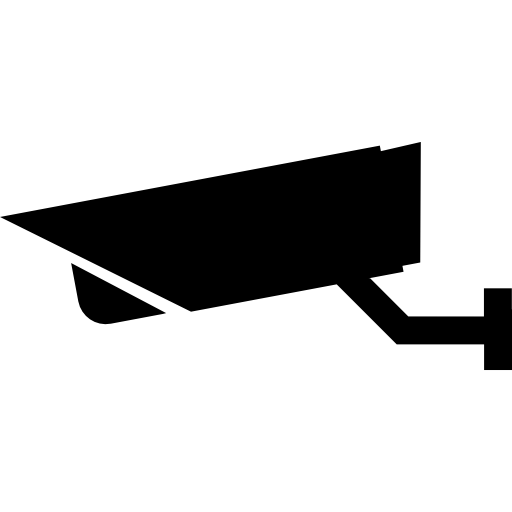
\includegraphics[width=.05\textwidth]{images/camera.png}};
		
		\node[above] at (2.2,2.6) {\scriptsize Raspberry Pi und Kamera};
		
		\node[inner sep=0pt] (whitehead) at (0,2)
		{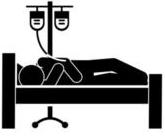
\includegraphics[width=.1\textwidth]{images/person_in_bed.png}};

			\node at (-2.6 ,-1) {ROOM VIEW};
	
			\draw [-, dashed, gray] (4,-0.5)-- (-4,-0.5)--(-4,-4) --(4, -4 ) --(4,-0.5);
		
		\node[inner sep=0pt] (whitehead) at (2,-1.5)
		{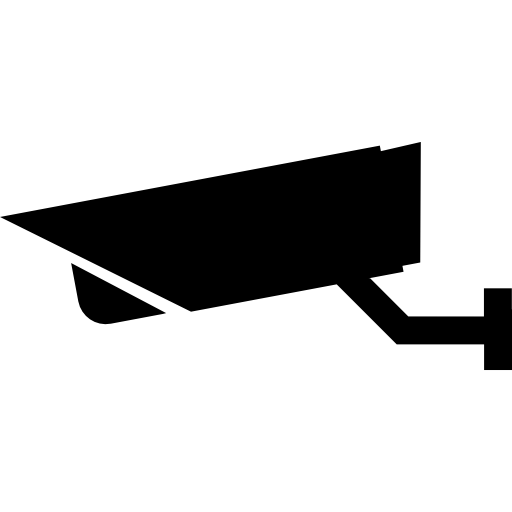
\includegraphics[width=.05\textwidth]{images/camera.png}};
		

		
		\node[inner sep=0pt] (whitehead) at (-0.25,-1.25)
		{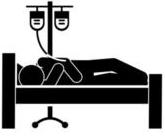
\includegraphics[width=.1\textwidth]{images/person_in_bed.png}};
		
		
		\node[inner sep=0pt] (whitehead) at (0,-2.25)
		{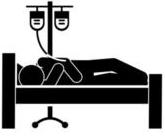
\includegraphics[width=.1\textwidth]{images/person_in_bed.png}};
		
	\node[inner sep=0pt] (whitehead) at (-0.5,-3.25)
		{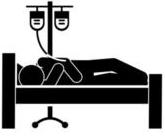
\includegraphics[width=.1\textwidth]{images/person_in_bed.png}};
		

	  \node[inner sep=0pt] (whitehead) at (4.0,0.25)
		{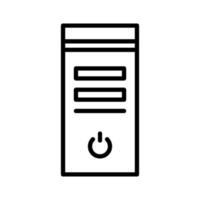
\includegraphics[width=.08\textwidth]{images/server.png}};
		
				\node[below] at (2.2,-1.6) {\scriptsize Raspberry Pi und Kamera};
		
		\node[below] at (4.0,-0.1) {\scriptsize MQTT Broker};
		
			
		
		\draw [-] (2,2.5)-- ( 3,2.5) -- (3,0.25) ;
		\draw [-] (2,-1.5)-- ( 3,-1.5) -- (3,0.25) ;
		\draw [-]  (3,0.25)  -- (3.8,0.25);

	    \draw [->]  (4.2 ,0.25) -- (5.0,0.25) -- (5.0,-1.5) -- (5.5,-1.5);
	     \draw [->]  (4.2 ,0.25) -- (5.0,0.25) -- (5.0,2.5) -- (5.5,2.5);
	
		\node at  (7.0,2.5) {Bed Detection};
		
		
		\node at  (7.0,-1.5) {Fall Detection};
		
		
	
	 	\draw [->]  (8.5 ,-1.5) -- (9.0,-1.5) -- (9,0.25) -- (9.5,0.25)  ;
	
		\draw [->]  (8.5, 2.5) -- (9.0,2.5) -- (9,0.25) -- (9.5,0.25) ;
		
		\node[inner sep=0pt] (whitehead) at (9.85,0.25)
		{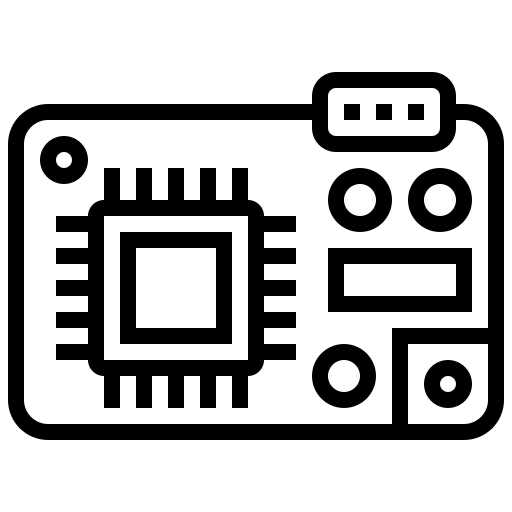
\includegraphics[width=.05\textwidth]{images/raspi.png}};
		
		\node[below] at (10.,0.1) {\scriptsize Raspberry Pi };
		
		\draw [->]  (10.3,0.25) -- (10.6,0.25) ;
		
		\node[red] at  (11.2,0.25) {Alarm};
		
		
	\end{tikzpicture}
	\caption{Darstellung des Systemaufbaus}
	\label{fig:patient_monitoring}
\end{figure}


\subsubsection{Fall Detektion}
In Abschnitt  \ref{sec:raspi} wurde bereits angerissen, dass ein Raspberry Pi mithilfe der Raspberry Pi Kamera eine Fall Detektion durchführen soll. Der Raspberry Pi soll also überprüfen, ob ein Patient hingefallen ist. Dies soll mithilfe des Yolo-Frameworks gemacht werden. Es ist hierbei Ziel das Modell auf dem Raspberry Pi zum Laufen zu bekommen, um möglichst nicht noch einen zusätzlichen Server zu benötigen. 

\subsubsection{Matrix}
Es soll einen Matrixserver geben. Über diesen Server sollen Pfleger auch auf dem Handy benachrichtigt werden, wenn eine Alarmsituation eingetreten ist. 


\subsection{Soll - Anforderungen}
\begin{itemize}
  \item Self-Hosted
  \item Alarm Licht
  \item Firewall (Router hat ja eh ne Firewall)
\end{itemize}

\subsubsection{Bett Detektion}
Es soll eine Komponente in unserem System geben, welche sich darum kümmert, zu erkennen, ob eine Person in einem Bett liegt. Es soll aber nicht jede Abwesenheit sofort zu einem Alarm führen, sondern nur, wenn über einen Zeitraum von 10 Minuten, das Bett leer bleibt, sollte ein Pfleger benachrichtigt werden, der dann nach dem Patienten schaut. Aufgrund der Zeitspanne von 10 Minuten, die das Bett leer bleiben muss, um einen Alarm auszulösen, ist es auch in Ordnung, wenn die Detektion etwas länger dauert. Es soll angestrebt werden, innerhalb von 30 Sekunden nach Verlassen des Betts zu erkennen das dieses leer ist. 

\subsection{Kann - Anforderungen}
\begin{itemize}
  \item QT-Kamera mit Kameraview
\end{itemize}

\subsection{MQTT Frontend}
Es kann ein MQTT - Frontend benutzt werden, um es Entwicklern einfacher zu machen die verschiedenen Nachrichten und Kommunikationskanäle nachzuvollziehen. 

\subsection{Gesprochene Information über Patient in Hilfesituation}
In den Minimalanforderungen unseres Systems weiß ein Pfleger nur das ein Patient Hilfe benötigt, nicht aber, welcher der Patienten. Um diese Problematik zu lösen, kann das System anstelle des Alarmtons über eine sprechende Stimme dem Pfleger mitteilen, welcher Patient Hilfe benötigt. 

\subsubsection{Kameraview}
Falls noch Zeit ist, soll zusätzlich mithilfe des QT-Frameworks eine Kameraview entwickelt werden. Mit dieser Anwendung sollen  Pfleger die Patienten überwachen können. Sie können so Dinge entdecken, die durch unsere Detektoren nicht abgedeckt werden. Ein Pfleger könnte so die Extubation eines Patienten erkennen. 
